\documentclass{article}

\usepackage{amsmath,amsfonts,amssymb,amsthm}
\usepackage{enumerate}
\usepackage{arydshln}
\usepackage{listings,color}
\usepackage{graphicx}

\definecolor{dkgreen}{rgb}{0,0.6,0}
\definecolor{gray}{rgb}{0.5,0.5,0.5}
\definecolor{mauve}{rgb}{0.58,0,0.82}

% Opening
\title{Numerical Analysis Project\\
Ch22 - 12 (pg)\\}
\author{Neal D. Nesbitt}

\begin{document}
\maketitle

\theoremstyle{definition}
\newtheorem{problem}{Problem}[section]
\newtheorem{solution}{Solution}[problem]
\renewcommand*{\thesolution}{\theproblem.\alph{solution}}

\lstset{basicstyle=\ttfamily,
		language=Matlab,
		keywordstyle=\color{blue},
		commentstyle=\color{dkgreen},
		stringstyle=\color{mauve},
		identifierstyle=\bf,
		numbers=left,
		numberstyle=\color{gray}
		}

\setcounter{section}{21}
\section{}

\setcounter{problem}{11}
\begin{problem}
Develop an M-File to solve a single ODE with the fourth order RK method. Design the M-file so that it creates a plot of the results. Test your program by using it to solve
\[ \frac{dy}{dx} = (1+4x)\sqrt{y} \]
with $x = 0$ to 1 using a step size of 0.1, where $y(0)=1$
\end{problem}

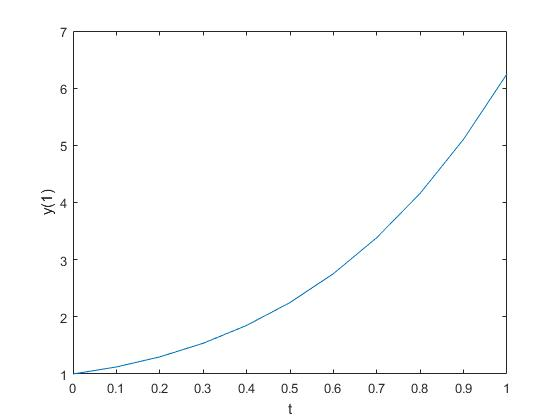
\includegraphics[width=\linewidth]{Project.jpg}

\begin{lstlisting}
function [ tp,yp ] = rk4ODEsysDisp( dydt,tspan,y0,h,varargin )
%% rk4ODEsysDisp: solves a system of first order ODEs, and plots the result
%   [ t,y ] = rk4sys( dydt,tspan,y0,h,varargin )
%       Uses the 4th order Runga Kutta method
%       to numerically solve a system of first order ODEs,
%       and then plot the results in both time and phase.
% input:
%   dydt = differential equation with independent(t) & dependent(y) inputs
%   tspan = [ti,tf]
%       ti = initial time
%       tf = final time
%   OR tspan = [ti,t1,t2...,tf] points to approximate the function at
%   y0 = initial values of dependent variables
%   h = step size
%   p1,p2,... = additional parameters used by dydt
% output:
%   tp = vector of independent variables
%   yp = vector of solution for dependent variables

%##########################################################################
%% Pseudo Code:
%   ####
%   Input Format Check:
%   ====
%   Variable Declarations:
%   ====
%   Main Algorithm:
%   ====
%   Plot Results:
%   ####
%##########################################################################
%% Input Format Check:

% Make sure all inputs are given,
if nargin<4
    error('ODE, time span, initial conditions, and step size required.');
end
% Make sure initial and final times are in increasing order
if any(diff(tspan)<=0),error('tspan not in ascending order');end

%==========================================================================
%% Variable Declarations:

m = length(y0);                 % Number of variables in the system
n = length(tspan);              % Number of steps between endpoints
ti = tspan(1); tf = tspan(n);   % Set variables first time and last time

% Setting up the steps for the time span:
% If the time span only contains an initial and final time,
if n==2
    t = (ti:h:tf)'; n = length(t);  % fill in the steps between.
    
    % If the last element didn't reach the final time
    if t(n)<tf
        t(n+1) = tf;    % Add an extra step
        n = n+1;
    end
else
    t = tspan; % Otherwise the times to approximate at are given explicitly
end

% Set up the other initial parameters for the method
tt = ti; y(1,:) = y0;
np = 1; tp(np) = tt; yp(np,:) = y(1,:);
i = 1;

%==========================================================================
%% Main Algorithm:

% For each given independent value:
while(1)
    tend = t(np+1);         % Set the current interval's end-point
    hh = t(np+1) - t(np);   % and the current interval's step size
    % 1 flop for setting the step size
    
    % If the time intervals were given explicitly, 
    % the current interval may be larger than the given step size.
    % If so, we adjust the step size and compute intermediate values.
    if hh>h, hh= h;end
    
    % Approximate the function value for the start of the next step:
    while(1)
        % If the step size overshoots the current interval,
        % then we also chop it down to fit
        if tt+hh>tend, hh = tend-tt;end
            % 1 or 2 flops, 
            % one for checking the interval and one for adjusting as needed
        
        % Start with the slope at the beginning of the step
        k1 = dydt(tt,y(i,:),varargin{:})';
            % dydt flops for computing the slope
        
        % Project k1 to get an estimate for the value of the function
        % at the midpoint of the step,
        ymid = y(i,:) + k1.*hh./2;        
        % and calculate the slope at this midpoint.
        k2 = dydt(tt+hh/2,ymid,varargin{:})';
            % 3m flops for projecting
            % 3 flops for setting the time value
            % dydt flops for computing the slope
        
        % Using the new slope k2, 
        % recalculate the projection at the midpoint
        ymid = y(i,:) + k2.*hh./2;        
        % and find another new slope k3.
        k3 = dydt(tt+hh/2,ymid,varargin{:})';
            % 3m flops for projecting
            % 3 flops for setting the time value
            % dydt flops for computing the slope
        
        % Using the last slope k3,
        % Re-project all the way to the end of the step
        yend = y(i,:) + k3.*hh;
        % and approximate the slope there.
        k4 = dydt(tt+hh,yend,varargin{:})';
            % 3m flops for projecting
            % 2 flops for setting the time value
            % dydt flops for computing the slope
        
        % Use the weighted RK4 formula to refine the approximation.
        phi = (k1 +2*(k2+k3) +k4)/6;
            % 5m flops for the final slope approximation
        
        % With the final slope approximation, project one more time 
        % to find the value of the function for the start of the next step
        y(i+1,:) = y(i,:) +phi*hh;
            % m+2 flops for projecting to the next step
        
        % Move to the next intermediate step in the approximation,
        % and break once we reach the next given time interval
        tt = tt+hh;
        i = i+1;
        if tt>=tend,break,end
            % 1 flop for moving to the next step
    end
    
    % Once we have reached the end of each time interval,
    % we record the values for output, and move to the next one.
    np = np+1; tp(np) = tt; yp(np,:) = y(i,:);
    
    % Once we hit the end of tspan, we break the loop.
    if tt>=tf,break,end
end

%==========================================================================
%% Plot Results

% Clear all current figures and turn off hold
cla
hold off

% Set up the grid of sub plots for each of the time and phase plots.
for i=1:(m^(2))
    sub(i) = subplot(m,m,i);
    set(sub(i),'Visible','off');
end

% Place each time plot solution in the left column.
for i=1:m
    subplot(sub(1+(i-1)*m)),plot(tp,yp(:,i));
    xlabel('t');
    ylabel(sprintf('y(%d)',i));
end

% Place phase graphs next to their corresponding time solutions
for i=1:m-1
    for j=i+1:m
        subplot(sub(((i-1)*m)+j)),plot(yp(:,j),yp(:,i));
        xlabel(sprintf('y(%d)',j));
        ylabel(sprintf('y(%d)',i));
    end
end
%##########################################################################
end
\end{lstlisting}

\end{document}